% IEEE standard conference template; to be used with:
%   spconf.sty  - LaTeX style file, and
%   IEEEbib.bst - IEEE bibliography style file.
% --------------------------------------------------------------------------

\documentclass[letterpaper]{article}
\usepackage{spconf,amsmath,amssymb,graphicx, hyphenat, hyperref}
\usepackage[skip=4pt]{caption}

% Example definitions.
% --------------------
% nice symbols for real and complex numbers
\newcommand{\R}[0]{\mathbb{R}}
\newcommand{\C}[0]{\mathbb{C}}
\newcommand{\abs}[1]{{\left\vert #1 \right\vert}}  %\abs{x} → |x|
\newcommand{\norm}[1]{{\left\Vert #1 \right\Vert}}  %\norm{x} → ||x||
\newcommand{\p}[1]{{\left( #1 \right)}}  %\p{x} → (x)
\newcommand{\brackets}[1]{{\left[ #1 \right]}}  %\b{x} → [x]
\newcommand{\braces}[1]{{\left\{ #1 \right\}}}  %\braces{x} → {x}
\newcommand{\ceil}[1]{{\left\lceil #1 \right\rceil}}  %\ceil{x} → ⌈x⌉
\newcommand{\floor}[1]{{\left\lfloor #1 \right\rfloor}}  %\floor{x} → ⌊x⌋
\newcommand{\mean}[1]{\operatorname{mean}\!\p{#1}}

% bold paragraph titles
\newcommand{\mypar}[1]{{\bf #1.}}

% Title.
% ------
\title{Polybench: optimizing doitgen and jacobi by hand}
%
% Single address.
% ---------------
\name{Antoine De Gendt, Quentin Guignard, Marie Jaillot, and Gilles Waeber} 
\address{Department of Computer Science, ETH Zürich\\Zürich, Switzerland}

% For example:
% ------------
%\address{School\\
%		 Department\\
%		 Address}
%
% Two addresses (uncomment and modify for two-address case).
% ----------------------------------------------------------
%\twoauthors
%  {A. Author-one, B. Author-two\sthanks{Thanks to XYZ agency for funding.}}
%		 {School A-B\\
%		 Department A-B\\
%		 Address A-B}
%  {C. Author-three, D. Author-four\sthanks{The fourth author performed the work
%		 while at ...}}
%		 {School C-D\\
%		 Department C-D\\
%		 Address C-D}
%

\setcounter{topnumber}{3}
\setcounter{bottomnumber}{1}
\setcounter{totalnumber}{4}
\renewcommand{\topfraction}{0.85}
\renewcommand{\bottomfraction}{0.85}
\renewcommand{\textfraction}{0.15}
\renewcommand{\floatpagefraction}{0.8}
\renewcommand{\textfraction}{0.1}
\setlength{\floatsep}{2pt plus 2pt minus 2pt}  % distance between floats on the top or the bottom and the text
\setlength{\textfloatsep}{5pt plus 2pt minus 2pt}  % distance between two floats
\setlength{\intextsep}{5pt plus 2pt minus 2pt}  % distance between floats inserted inside the page text (using h) and the text proper

\def\NR{{\rm NR}}
\def\NQ{{\rm NQ}}
\def\NP{{\rm NP}}

\begin{document}
%\ninept
%
\maketitle
%

%The hard page limit is 6 pages in this style. Do not reduce font size
%or use other tricks to squeeze. This pdf is formatted in the American letter format, so the spacing may look a bit strange when printed out.

\begin{abstract}
%Describe in concise words what you do, why you do it (not necessarily
%in this order), and the main result.  The abstract has to be
%self-contained and readable for a person in the general area. You
%should write the abstract last.
%\the\columnwidth (divide by 72.27 to get in inches = 3.287in)
%\the\textheight (divide by 72.27 to get in inches = 8.897in)
We present here implementation concepts optimized for parallelism for selected polybench algorithms: doitgen, jacobi1d and jacobi2d.
We explore both a thread-level parallelization using OpenMP and process-level parallelization using MPI to determine the main optimization axis for those problems.
\end{abstract}

\section{Introduction}\label{sec:intro}
\mypar{Motivation} The goal of this project is to optimize and parallelize benchmarks in the Polybench benchmark suite in order to give a baseline for "human" optimization. We chose the Doitgen kernel and the Jacobi stencil because they represent real world problems and common workloads. Today, parallelization is necessary to fully exploit the capabilities of the hardware. Two APIs will be used : OpenMP and MPI\footnote{Message Passing Interface}. Our main contribution is a baseline for comparison.

\mypar{Related work}
%\footnote{\href{https://web.cse.ohio-state.edu/~pouchet.2/software/polybench/}{Polybench 4.1}}
Polybench\cite{polybench} provides simple sequential implementations for these algorithms. In \cite{data-centric-python}, some of these benchmarks are automatically parallelized.


%Do not start the introduction with the abstract or a slightly modified
%version. It follows a possible structure of the introduction. 
%Note that the structure can be modified, but the
%content should be the same. Introduction and abstract should fill at most the first page, better less.

%\mypar{Motivation} The first task is to motivate what you do.  You can
%start general and zoom in one the specific problem you consider.  In
%the process you should have explained to the reader: what you are doing,
%why you are doing, why it is important (order is usually reversed).

%For example, if my result is the fastest sorting implementation ever, one
%could roughly go as follows. First explain why sorting is important
%(used everywhere with a few examples) and why performance matters (large datasets,
%realtime). Then explain that fast implementations are very hard and
%expensive to get (memory hierarchy, vector, parallel). 

%Now you state what you do in this paper. In our example: 
%presenting a sorting implementation that is
%faster for some sizes as all the other ones.

%\mypar{Related work} Next, you have to give a brief overview of
%related work. For a report like this, anywhere between 2 and 8
%references. Briefly explain what they do. In the end contrast to what
%you do to make now precisely clear what your contribution is.

\section{Background: Selected Algorithms}\label{sec:background}
\mypar{Doitgen} This algorithm is performing a series of matrix matrix multiplication given $A\in\R^{{\rm NR}\times {\rm NQ} \times {\rm NP}}$ and $C4\in\R^{{\rm NP}\times {\rm NP}}$ and is defined as $A(r, q, p) = \sum_{\substack{s=0}} A(r, q, s)*C4(s, p)$.

\mypar{Stencil algorithms} Those where we repeatedly update values in an array according to a pattern, i.e.~stencil.
Parallel implementations of such algorithms are challenging due to the coupling between a cell and its neighbors.
The dependency on the previous value of the cell itself also prevents parallelizing over the time.

\mypar{Jacobi 1D} Given an array $A\in\R^n$ and a number of steps $t$, we replace $t$ times $A$ with $A'$ with $A'_1=A_1, A'_n=A_n, A'_i=\mean{A_{i-1},A_{i},A_{i+1}}$ for $i\not\in\braces{1,n}$.

\mypar{Jacobi 2D} Given a 2D array $A\in\R^{n\times n}$ and a number of steps $t$, we replace $t$ times $A$ with $A'$ with $A'_{i,j}=A_{i,j}$ for $i\in\braces{1,n}\lor j\in\braces{1,n}$, i.e.~the border cells, and
$A'_{i,j}=\mean{A_{i,j},A_{i-1,j},A_{i+1,j},A_{i,j-1},A_{i,j+1}}$ otherwise.

\mypar{Verification} To ensure the correctness of the proposed implementation, we tested against the reference Polybench code.

\mypar{Generating data} To generate the data, we collected 10 runs for each parameter modification. Then, the data was plotted using functions provided in the R scripts of the LibSciBench \cite{libscibench} repo.

%Give a short, self-contained summary of necessary
%background information. For example, assume you present an
%implementation of sorting algorithms. You could organize into sorting
%definition, algorithms considered, and asymptotic runtime statements. The goal of the
%background section is to make the paper self-contained for an audience
%as large as possible. As in every section
%you start with a very brief overview of the section. Here it could be as follows: In this section 
%we formally define the sorting problem we consider and introduce the algorithms we use
%including a cost analysis.

%\mypar{Sorting}
%Precisely define sorting problem you consider.

%\mypar{Sorting algorithms}
%Explain the algorithm you use including their costs.

%As an aside, don't talk about "the complexity of the algorithm.'' It's incorrect,
%problems have a complexity, not algorithms.


\section{Experimental Setup}\label{sec:experimental_setup}
All our benchmarks are run on Euler VII nodes (CPU:
\href{https://www.amd.com/fr/products/cpu/amd-epyc-7h12}{AMD EPYC 7H12}, 64 cores).
For this project, we were limited to 48 cores and could not obtain exclusive access to a node, which means other jobs could potentially be using the same nodes at the same time, affecting the results.
The software stack is gcc/9.3.0+openmpi/4.0.2.
Compilation options were -O3 -mavx2 -mfma.
Unless otherwise specified, each experiment was run 10~times.

\section{Doitgen}\label{sec:doitgen}

\subsection{OpenMP}\label{sec:doitgenOpenMp}

\begin{figure}
  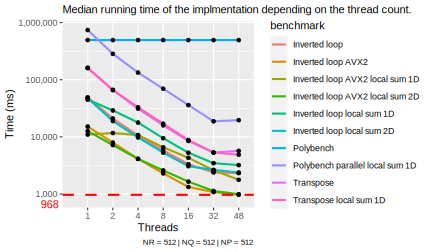
\includegraphics[scale=0.54]{Doitgen_OpenMP/classic_data_plot.eps}
  \caption{Comparisons of several implementations for Doitgen.}
  \label{fig:doitgen_openmp_classic_data}
\end{figure}

\begin{figure}
  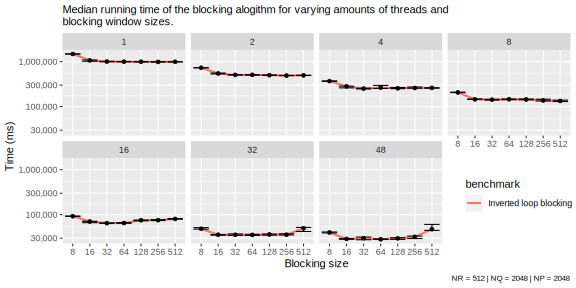
\includegraphics[scale=0.41]{Doitgen_OpenMP/blocking_data_scale_plot.eps}
  \caption{Study of the blocking algorithm with different parameters. Each plot corresponds to a specific number of threads.}
  \label{fig:doitgen_openmp_blocking_scale_data}
\end{figure}

\begin{figure}
  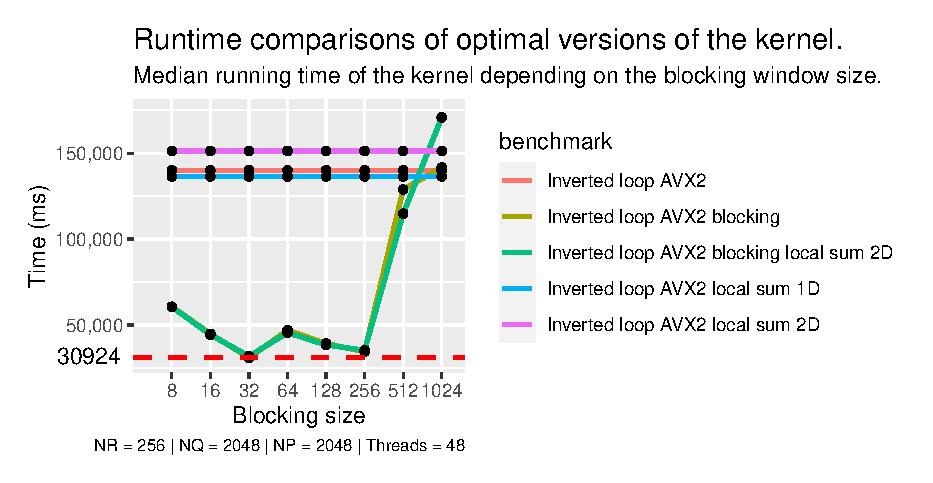
\includegraphics[scale=0.54]{Doitgen_OpenMP/optimized_data_plot.eps}
  \caption{The dashed line represents the smallest running time.}
  \label{fig:doitgen_openmp_optimized_data}
\end{figure}

\begin{figure}
  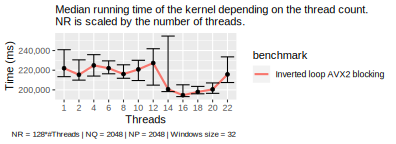
\includegraphics[scale=0.59]{Doitgen_OpenMP/scaling_data_plot.eps}
  \caption{Study of the inverted loop AVX2 blocking implementation with scaling.}
  \label{fig:doitgen_openmp_scaled_data}
\end{figure}

\subsubsection{Proposed methods}\label{proposed_methods_openmp}

In this section, we will talk about the parallelization and optimization of the doitgen kernel using the Open\hyp{}MP API. We parallelized Doitgen as follows : one thread computes a sequence of \textbf{complete} matrix-matrix multiplications. More concretely, the parallelism occurs along the NR axis of the input matrix. To extract the most performance out of our CPU, we need to leverage the cache. To explore the impact of better cache utilization, we implemented a version of the algorithm that uses a transposed C4 matrix, a version where the two inner loops are inverted and a blocking version.

\mypar{Local sum} The initial version of the kernel provided by Polybench does not use an input and output matrix, only an input matrix is used. Then, in the kernel, the elements of a resulting line are incrementally built up and stored into an array that is then put back in the input matrix.
This way of performing the computation consumes $\NR\times\NQ\times\NP + \NP$ memory rather than $2\times\NR\times\NQ\times\NP$ when an output matrix is used. The difference between the versions with a local sum array and without will be explored in the following section.
Also, in the parallel algorithms, each thread has its own sum array, resulting in a ${\rm\#Threads}\times\NP$ table when a 1D sum array is used and in a ${\rm\#Threads}\times\NQ\times\NP$ table when a 2D sum array is used.

\mypar{Transpose version} In this version, the C4 matrix is transposed, it is thus traversed row by row.

\mypar{Inverted loops version} We incrementally build the elements of a line of the output matrix by traversing A by rows and C4 by rows. Then, we switch to another line of C and another line of A to build the elements of another line of the output matrix.

\mypar{Blocking version} In the blocking version of the kernel, the goal is to reuse values brought in from cache as much as possible. This is achieved by multiplying sub-matrices rather than multiply one matrix with another at once. This improvement can be combined with one of the two mentioned previously. As currently implemented, this version only works if the blocking size divides the matrix size.

\mypar{Vectorization}
The vectorization version of the kernel uses the AVX2 and FMA instruction sets. The AVX2 instruction set deals with 256 bits registers, allowing us to load doubles (8 bytes) 4 by 4. As currently implemented, this version only works if the matrix row size is divisible by 4.

\subsubsection{Experimental results}\label{experimental_results_openmp}
Here, results of the benchmarking of the different implementations will be presented.

\mypar{Finding the best implementation}
First, we decided to benchmark all the implementations with a rather small matrix size to see what the fastest were. See Figure \ref{fig:doitgen_openmp_classic_data} (beware of the logarithmic scale). We clearly see that the inverted loop AVX2 implementations are the fastest ones.

\mypar{Blocking window size}
Now, we want to know if pursuing blocking is worth it and how it performs under different blocking window sizes and varying amounts of threads. The results are available in Figure \ref{fig:doitgen_openmp_blocking_scale_data}. We see that the higher the thread count the higher the impact of blocking on performance. This may be because this allows for threads to work on different parts of the matrix, causing less cache coherency traffic and less cache associativity issues.

\mypar{Finding the best version}
With this data we can now conclude that an inverted loop AVX2 implementation with blocking should yield the best results. The outcome of this experiment is available in Figure \ref{fig:doitgen_openmp_optimized_data}.
Blocking improves greatly the performance of the algorithm. It seems to have a greater impact than on single threaded applications. The benchmarks appearing on the figure that do not use blocking were not run for each blocking size, they should be read as constant straight lines. Also, the 1D local sum version seems to be faster than the other two. This may be explained by cache coherency traffic, cache associativity and lower memory consumption. In Figure ~\ref{fig:doitgen_openmp_scaled_data}\footnote{We didn't manage to plot for greater thread counts(the limit is 22) because of memory consumption issues.}, the running time varies around 220s for different amounts of threads. This may be because the chosen window size is tailored to work well with 48 threads but not necessarily for other thread counts.

\subsection{MPI}\label{sec:doitgenMPI}

\subsubsection{Proposed methods}\label{proposed_methods_doitgenmpi}

In this section we will briefly describe how Doitgen was parallelized with MPI. After that, we will describe our three experiments.

We parallelized Doitgen very similarly as in the OpenMP section.
We split the work among processes by attributing to each process a chunk of matrices along the NR axis. Each process is allocating a batch of 64 $\NQ\times\NP$ matrices.
It is worth to note that the initial problem size is $128\times512\times512$ and that we scaled the NR axis with the number of processes. Moreover, our algorithm works in three phases, firstly it initializes A. The second phase is the kernel execution (a full batch in a row). Finally, the last phase consists of writing the batch to a remote location. Note that there is no network communication except when writing the batch. Now that we described our algorithm, let's talk about our experiments.

We made a total of three experiments. The first experiment consisted of comparing four writes strategies along two axis, using or not collective writes and using or not a file window. This was done in order to choose the simplest best write strategy. Secondly, we compared the runtime of each phases of our algorithm and we proposed an improvement by transposing the slices in place before the execution of the kernel. We measured each phases as well as the overall runtime. We also reported the sequential baseline\footnote{We used the Doitgen implementation of \href{https://web.cse.ohio-state.edu/~pouchet.2/software/polybench/}{Polybench 4.1} }. Finally, we observed the effect of spanning multiple nodes and measured everything exactly as in the second experiment. Now that we have described our experiments, let's see our results.

\subsubsection{Experimental results}\label{experimental_results_mpi}

In this section we will report and discuss our experiments results. We will start with the write strategy.

When comparing the 4 different strategies, we can ask ourselves how much the 4 write strategies affect the runtime. By looking at Figure \ref{fig:doitgen_mpi_write_strategy} we can observe that there are two trends, the collective writes are slower than the individual writes and using a window does not affect the results at all. This result follows are intuition since the write regions are disjoints per process and any collective calls imply some synchronization overhead. We therefore choose an individual call and we are now able to compare the proportion of each phase runtime in our second experiment.


\begin{figure}
  \includegraphics[scale=0.40]{Doitgen_MPI/write_2.pdf}\hfill
  \caption{}
  \label{fig:doitgen_mpi_write_strategy}
\end{figure}


Indeed, we need to know which phase dominates the runtime in order to make things faster.
\begin{figure}
  \includegraphics[scale=0.60]{Doitgen_MPI/latest_plots/grapix_kernel.pdf}\hfill
  \caption{Runtime of a single iteration of the kernel. Median time per process per iteration for each process number}
  \label{fig:doitgen_mpi_kernel_basic}
\end{figure}

\begin{figure}
  \includegraphics[scale=0.52]{Doitgen_MPI/latest_plots/write_no_title.pdf}\hfill
  \caption{Runtimes of a batch write. All time measurements per process per iteration for each process number}
  \label{fig:doitgen_mpi_write_basic}
\end{figure}

\begin{figure}
  \includegraphics[scale=0.50]{Doitgen_MPI/latest_plots/overall_no_title.pdf}\hfill
  \caption{Overall runtimes with baseline. Median time of the median process runtime per run for each process number.}
  \label{fig:doitgen_mpi_overall_basic}
\end{figure}

First, by looking at the \textit{basic} versions of Figure \ref{fig:doitgen_mpi_overall_basic}, we can observe that the runtime of the algorithm is about 125 seconds and match the baseline as expected. We did not included the plot for the phase 1 because it was always taking around $75 ms$ and was therefore insignificant to the rest. For the second phase on Figure \ref{fig:doitgen_mpi_kernel_basic}, we can see that the basic kernel takes about $900 ms$ per iteration. For the third phase on Figure \ref{fig:doitgen_mpi_write_basic} and by looking at the basic violin, we can observe that a single batch write can take up to 10 seconds. Therefore, since there is only two write of batch per process and 128 kernel iterations per process, the overall runtime is dominated by the kernel execution. With this information in mind, we introduce an improvement. Indeed, similarly as in the openMP version, we could ask us how much would the kernel benefits from friendlier memory accesses. In order to answer this question we transposed the batch in place before executing the kernel. We first noted that the phase 1 runtime remained unchanged even with the transposition (still not showed). Secondly, we noted a performance improvement as it can be observed by looking at both the \textit{basic} and \textit{transposed} version on Figure \ref{fig:doitgen_mpi_kernel_basic} where a single kernel iteration dropped to around $200 ms$ and the overall runtime dropped to around $20s$ of runtime. We won't cover much about the cache issues and why its faster as it is already done in the OpenMP section. However, we can note a progressive overhead in the runtime in the \textit{transpose} version still on Figure \ref{fig:doitgen_mpi_overall_basic} as the number of processes increases.Could this be the cache? Interestingly, we don't observe the same progressive overhead on each kernel iterations runtime on Figure \ref{fig:doitgen_mpi_kernel_basic} therefore the kernel phase is not at the origin of this overhead. What about the writes? Indeed, we observe a change on Figure \ref{fig:doitgen_mpi_write_basic}, the more nodes we span, the lower the clusters are located which indicates that the writes took less time (Note the logarithmic scale). This progressive overhead could be due from either network bandwidth sharing, from cache contention (not in the kernel) or from disk contention.The latter can be excluded because if this was the disk, spanning more nodes would have no effect. This let us with the network and cache contention in another phase than 2. As said previously, the phase 1 was taking around $200ms$ for a single batch and therefore cannot be guilty for the overhead. We don't see another place where cache contention could build up except in the write because we don't know the implementation of the MPI write. Perhaps MPI is sharing memory for the processes on same node which would incure an overhead when lots of processes are on the same node? Unfortunately, we don't have any experiment for that but that could be aligned with Figure \ref{fig:doitgen_mpi_write_basic} and would explain the speed up when spanning more nodes. Lastly, it could be the network bandwith sharing from the node to the remote write location. However, doing an approximate computation leads to 200ms per iteration and 64 iteration to write $1072Mbit$ (a batch) imply $89Mbit/s$ and at most $4288Mbit/s$ with 48 processes. This is far from the $100GBits$ bandwith in euler VII to scratch location and therefore could explain the overhead in Figure \ref{fig:doitgen_mpi_overall_basic}, the speed ups in writes on Figure \ref{fig:doitgen_mpi_write_basic} and the absence of overhead on Figure \ref{fig:doitgen_mpi_kernel_basic}.
To conclude, we could optimize and provide a human optimization for Doitgen implemented with MPI but we cannot explain precisely the reason of the overhead except with the above given ideas. One sure thing is that this overhead is due to something on the node, either the network or the cache. Let's now switch to Jacobi.





%Now comes the ``beef'' of the report, where you explain what you
%did. Again, organize it in paragraphs with titles. As in every section
%you start with a very brief overview of the section.

%In this section, structure is very important so one can follow the technical content.

%Mention and cite any external resources that you used including libraries or other code.

\section{Jacobi}

\subsection{OpenMP}
\begin{figure}
  \includegraphics{jacobi_omp/1d_scaling.pdf}
  \caption{Jacobi 1D: execution time per number of threads, with $N = 10 000 *$ number of threads}
  \label{fig:j1d_scaling}
\end{figure}
\begin{figure}
  \includegraphics{jacobi_omp/2d_scaling.pdf}
  \caption{Jacobi 2D: execution time per number of threads, with $N = 100 *$ number of threads}
  \label{fig:j2d_scaling}
\end{figure}

\subsubsection{Proposed methods}\label{jacobi_openmp_methods}
In this section, we will present the different parallelizations of Jacobi 1D and 2D achieved with OpenMP.

\mypar{Jacobi 1D} Since Jacobi iteratively updates the cells of the given array $A$, we could not parallelize the execution of all the time steps. We thus only parallelized the computation of each cell’s new value within a single time step. The first loop, which performs the computation over the cells of array $A$ and stores them in a second array $B$, is divided between all threads and once this computation is finished, the second loop is also split between the threads to update $A$ with these new values. Another more efficient method was to replace the second loop, responsible for transferring the values from array $B$ to array $A$, with a simple swap between the two array pointers.

\mypar{Jacobi 2D} With Jacobi 2D the parallelizations were done in the same fashion. The time steps are executed sequentially and for each time step, the computation of the new values is parallelized over the two dimensions. Again, another optimization was achieved by replacing the transfer of values between matrix $A$ and $B$ by a swap of pointers.

\subsubsection{Experimental results}\label{experimental_results_jacobi_openmp}
We will now discuss the benchmark results of our different implementations.
To test the efficiency of our implementation, we performed 10 runs for each execution parameter set. We used 1000 time steps and an array size of $N = 10 000$ and $N = 100$ for Jacobi 1D and 2D respectively, multiplied by the number of processes. In Figure \ref{fig:j1d_scaling} with Jacobi 1D, we see that the two parallelizations achieved better performances, especially the implementation using the pointer swap mentioned above. For Jacobi 2D in Figure \ref{fig:j2d_scaling} the two parallelizations were just as efficient and scale well.

\subsection{MPI}
\begin{figure}
  \includegraphics{jacobi_mpi/1d_halo.pdf}
  \caption{Jacobi 1D MPI: comparing halo depths}
  \label{fig:j1d_halo}
\end{figure}
\begin{figure}
  \includegraphics{jacobi_mpi/1d_nodes.pdf}
  \caption{Jacobi 1D MPI: spanning multiple nodes}
  \label{fig:j1d_nodes}
\end{figure}
\begin{figure}
  \includegraphics{jacobi_mpi/2d_multi.pdf}
  \caption{Jacobi 2D MPI: comparing program variants}
  \label{fig:j2d_multi}
\end{figure}
\begin{figure}
  \includegraphics{jacobi_mpi/2d_vhalo.pdf}
  \caption{Jacobi 2D MPI: halo depth for vstack}
  \label{fig:j2d_vhalo}
\end{figure}

\subsubsection{Proposed methods}\label{jacobi_mpi_methods}
For Jacobi MPI implementations, we assume that each process should only store a small part of the complete array in its memory.
Given the dependency between a cell and its neighbors, we need to share data between the different processes, a solution being to share data with the neighboring processes when necessary.

\mypar{Ghost Cells} An applicable pattern here are ghost cells \cite{ghost_cells}.
We store a padded array, slightly larger than the array to compute, and only compute the values of the cells in the central part while the cells at the borders are computed by other processes and exchanged whenever necessary.
Concretely, for Jacobi 1D, we store an additional cell at the beginning and at the end of the array, and
after every iteration, each process sends the first and the last values it computed to the previous resp.~next process, which uses it to update its border cells.

\mypar{Deep Halo} Extending on the idea of ghost cells, we store a bigger array to reduce the number of inter-process data exchanges required.
Thus, data packets are bigger and the relative data transfer overhead is reduced.
As the stencil must now also be applied on some border cells too, the total computation increases.
We define the halo depth as the number of iterations between every data exchange, equal here to the number of additional ``padding'' cells on each side of the array.
Ghost cells correspond to a depth of $1$.
A depth greater than the number of iteration means that no data exchange is necessary.
Data exchange and computation overhead must be balanced.
Greater depth could lead to data exchanges with processes further away.

\mypar{Striped Synchronization} To avoid unnecessary wait times, we use striped synchronization: we number all processes sequentially, then processes with an odd number start by synchronizing with their previous neighbor and those with an even number start by synchronizing with their next neighbor.

\mypar{2-Step Synchronization}
For Jacobi 2D, we can cut the area as a grid.
With the deep halo approach, each process would need to exchange data with up to 8 neighbors.
Due to the grid structure, data between processes in diagonal is small and also passed to their two common neighbors.
An alternative is a two-step synchronization: first vertically only, then horizontally also passing corners' data whenever relevant.
This introduces an additional wait, but reduces the number of communication channels.

\mypar{Stacked processes}
Instead of disposing processes' areas in a grid, we simply divide the space over one axis, e.g.~vertically.
This reduces the number of neighbor for each process but the total amount of data exchanged increases.


\subsubsection{Experimental results}\label{jacobi_mpi_results}
Problem sizes were scaled using the number of cores used (denoted $S$) as in \cite{data-centric-python}.
Unless for varying the number of node, each experiment was run as a single batch.
All experiments use striped async data exchange.
Striped vs. non-striped did not make a significant difference.

\mypar{Jacobi 1D}
In Fig.~\ref{fig:j1d_halo}, we examine the effect of deep halo on the computation time.
Looking especially at the depths of $1$ and $8$, we see that the runtime is halved when using 48 cores.
For 8 cores or more, we see that using a depth between 4 and 32 produces particularly stable results.
In Fig.~\ref{fig:j1d_nodes}, we compare the runtimes for different number of nodes, to check if any adversary effect occurs when spanning the cores over more nodes.
To the contrary, spanning over more nodes seems to decrease runtimes.
While this may be caused by under-utilization of the specific processes in the cluster, it demonstrates that the proposed implementation scales properly with nodes.

\mypar{Jacobi 2D}
Since the array has size $N^2$, we scale the problem to $N=1000\sqrt S$.
In Fig.~\ref{fig:j2d_multi}, we compare the different implementation: diagonal sync, 2-step sync, and stacked processes for different halo depths.
The stacked processes implementation scales better than the other two, despite exchanging more data between the processes.
It is however greatly affected by the halo depth.
The 2-step and base (diagonal sync) implementation seem to be roughly on par.
The effects of varying halo depth are weaker.
% vstack: $2\cdot T\cdot G\cdot S\cdot N$
% diag: $2\cdot T\cdot G\cdot 2\sqrt S\cdot N + 8(\sqrt S-1)^2\frac{G\cdot (G-1)}{2}$
% 2-step: $2\cdot T\cdot G\cdot 2\sqrt S\cdot N + 4(\sqrt S-1)^2\frac{G\cdot (G-1)}{2}$
In Fig.~\ref{fig:j2d_vhalo}, we focus on the latter to determine the best halo depth.
Between 4 and 8 seems optimal in our case.

%\section{Experimental Results}\label{sec:jacobi_mpi_exp}

%Here you evaluate your work using experiments. You start again with a
%very short summary of the section. The typical structure follows.

%\mypar{Experimental setup} 
%Specify the platform (processor, frequency, maybe OS, maybe cache sizes)
%as well as the compiler, version, and flags used. If your work is about performance, 
%I strongly recommend that you play with optimization flags and consider also icc for additional potential speedup.

%Then explain what kind of benchmarks you ran. The idea is to give enough information so the experiments are reproducible by somebody else on his or her code.
%For sorting you would talk about the input sizes. For a tool that performs NUMA optimization, you would specify the programs you ran.

%\mypar{Results}
%Next divide the experiments into classes, one paragraph for each. In each class of experiments you typically pursue one questions that then is answered by a suitable plot or plots. For example, first you may want to investigate the performance behavior with changing input size, then how your code compares to external benchmarks.

%For some tips on benchmarking including how to create a decent viewgraph see pages 22--27 in \cite{Pueschel:10}.

%{\bf Comments:}
%\begin{itemize}
%\item Create very readable, attractive plots (do 1 column, not 2 column plots
%for this report) with readable font size. However, the font size should also not be too large; typically it is smaller than the text font size.
%An example is in Fig.~\ref{fftperf} (of course you can have a different style).
%\item Every plot answers a question. You state this question and extract the
%answer from the plot in its discussion.
%\item Every plot should be referenced and discussed.
%\end{itemize}

%\begin{figure}\centering
  %\includegraphics[scale=0.33]{dft-performance.eps}
%  \includegraphics[scale=0.25]{test.pdf}
%  \caption{Performance of four single precision implementations of the
%  discrete Fourier transform. The operations count is roughly the
%  same. The labels in this plot are maybe a little bit too small.\label{fftperf}}
%\end{figure}

\section{Conclusions}
We managed to provide manual optimizations that improves well over the base sequential implementations. This was done using different techniques.

\mypar{Doitgen}
We observed scalable results for both Open\hyp{}MP and MPI using different techniques. We found that the combination of vector instructions, blocking and inverting the loops for matrix-matrix multiplication yielded the best results. For MPI we found that using individual write calls would yield good results over collective calls. We also verified that doitgen could easily span multiple nodes. One possible improvement would be to apply all the OpenMP techniques to the MPI version.


\mypar{Jacobi} Despite the challenge of the algorithm, we were able to parallelize it using both OpenMP and MPI.
For OpenMP, the most efficient was combining a pointer swap with a classic parallelization of the computation loop. Exploring overlapped tiling might provide better improvements.
For MPI, using deep halo techniques provided to most important improvement.
We believe that it would be possible to obtain even better results by reorganizing the memory accesses s.t.~the local part that is being worked on fits in cache.
The 2-step synchronization performed less well in our test.
Another way to reduce data exchange overhead would be to let synchronizations happen at the same time as we compute other parts of the matrices, which however greatly improves code complexity.


%Here you need to summarize what you did and why this is
%important. {\em Do not take the abstract} and put it in the past
%tense. Remember, now the reader has (hopefully) read the report, so it
%is a very different situation from the abstract. Try to highlight
%important results and say the things you really want to get across
%such as high-level statements (e.g., we believe that .... is the right
%approach to .... Even though we only considered x, the
%.... technique should be applicable ....) You can also formulate next
%steps if you want. Be brief. After the conclusions there are only the references.

%\section{Further comments}

%Here we provide some further tips.

%\mypar{Further general guidelines}

%\begin{itemize}
%\item For short papers, to save space, I use paragraph titles instead of
%subsections, as shown in the introduction.

%\item It is generally a good idea to break sections into such smaller
%units for readability and since it helps you to (visually) structure the story.

%\item The above section titles should be adapted to more precisely
%reflect what you do.

%\item Each section should be started with a very
%short summary of what the reader can expect in this section. Nothing
%more awkward as when the story starts and one does not know what the
%direction is or the goal.

%\item Make sure you define every acronym you use, no matter how
%convinced you are the reader knows it.

%\item Always spell-check before you submit (to us in this case).

%\item Be picky. When writing a paper you should always strive for very
%high quality. Many people may read it and the quality makes a big difference.
%In this class, the quality is part of the grade.

%\item Books helping you to write better: \cite{Higham:98} and \cite{Strunk:00}.

%\item Conversion to pdf (latex users only): 

%dvips -o conference.ps -t letter -Ppdf -G0 conference.dvi

%and then

%ps2pdf conference.ps
%\end{itemize}

%\mypar{Graphics} For plots that are not images {\em never} generate the bitmap formats
%jpeg, gif, bmp, tif. Use eps, which means encapsulate postscript. It is
%scalable since it is a vector graphic description of your graph. E.g.,
%from Matlab, you can export to eps.

%The format pdf is also fine for plots (you need pdflatex then), but only if the plot was never before in the format 
%jpeg, gif, bmp, tif.


% References should be produced using the bibtex program from suitable
% BiBTeX files (here: bibl_conf). The IEEEbib.bst bibliography
% style file from IEEE produces unsorted bibliography list.
% -------------------------------------------------------------------------
\bibliographystyle{IEEEbib}
\bibliography{bibl_conf}

\nocite{MPItutorials}
\nocite{MPIForDummies}
\nocite{MPIIOBestPracice}
\nocite{cache_lec}

\end{document}

